\documentclass[12pt,reqno, twoside]{amsbook}
%%%%%%%%%%%%%%%%%%%%%%%%%%%%%%%%%%%%%%%%%%%%%%%%%%%%%%%%%%%%%%%%%%%%%%%%%%%%%%%%%%%%%%%%%%%%%%%%%%%%%%%%%%%%%%%%%%%%%%%%%%%%%%%%%%%%%%%%%%%%%%%%%%%%%%%%%%%%%%%%%%%%%%%%%%%%%%%%%%%%%%%%%%%%%%%%%%%%%%%%%%%%%%%%%%%%%%%%%%%%%%%%%%%%%%%%%%%%%%%%%%%%%%%%%%%%
\usepackage{eurosym}
\usepackage{amsmath}
\usepackage{amssymb}
\usepackage{amsfonts}
\usepackage[onehalfspacing]{setspace}
\usepackage{chngcntr}
\usepackage{graphicx}
\usepackage[a4paper, margin=2.5cm]{geometry}
\usepackage[english]{babel}
\usepackage{fancyhdr}
\usepackage{titlesec}
\usepackage{enumitem}
\usepackage{etoolbox}
\usepackage{csquotes}
\usepackage[printonlyused]{acronym}
%
% you may need to uncomment the command below if you use eps format for figures
%\usepackage{epstopdf}
%
\usepackage[
    backend=biber,
    style=ieee,
  ]{biblatex}
\addbibresource{references.bib}
%
\makeatletter
    \def\section{\@startsection{section}{1}%
      \z@{.5\linespacing\@plus.7\linespacing}{.25\linespacing}%
      {\normalfont\bfseries\flushleft}}
    \def\subsection{\@startsection{subsection}{2}%
      \z@{.5\linespacing\@plus.7\linespacing}{.25\linespacing}%
      {\normalfont\bfseries\flushleft}}
%
\makeatother
\setcounter{MaxMatrixCols}{10}
%
\providecommand{\U}[1]{\protect\rule{.1in}{.1in}}
\theoremstyle{plain}
\newtheorem{acknowledgement}{Acknowledgement}
\newtheorem{algorithm}{Algorithm}[chapter]
\newtheorem{axiom}{Axiom}[chapter]
\newtheorem{case}{Case}[chapter]
\newtheorem{claim}{Claim}[chapter]
\newtheorem{conclusion}{Conclusion}[chapter]
\newtheorem{condition}{Condition}[chapter]
\newtheorem{conjecture}{Conjecture}[chapter]
\newtheorem{corollary}{Corollary}[chapter]
\newtheorem{criterion}{Criterion}[chapter]
\newtheorem{definition}{Definition}[chapter]
\newtheorem{example}{Example}[chapter]
\newtheorem{exercise}{Exercise}[chapter]
\newtheorem{lemma}{Lemma}[chapter]
\newtheorem{notation}{Notation}[chapter]
\newtheorem{problem}{Problem}[chapter]
\newtheorem{proposition}{Proposition}[chapter]
\newtheorem{remark}{Remark}[chapter]
\newtheorem{solution}{Solution}[chapter]
\newtheorem{summary}{Summary}[chapter]
\newtheorem{theorem}{Theorem}[chapter]
\numberwithin{equation}{chapter}
%
\makeatletter
\newcommand\frontFont{\@setfontsize\frontFont{14.4}{14.4}}
\makeatother
%
% Please write the references according to your school
%
\newenvironment{dedication}
  {%\clearpage           % we want a new page
   \thispagestyle{empty}% no header and footer
   \vspace*{\stretch{1}}% some space at the top
   \itshape             % the text is in italics
   \raggedleft          % flush to the right margin
  }
  {\par % end the paragraph
   \vspace{\stretch{3}} % space at bottom is three times that at the top
   %\clearpage           % finish off the page
  }
  \numberwithin{section}{chapter}
\fancyhead{}
\fancyfoot{}
\pagestyle{fancy}
\fancyfoot[LE,RO]{\thepage}
%
\makeatletter
\def\ps@plain{\ps@empty
 \def\@evenfoot{%
   \normalfont\scriptsize
   \rlap{\thepage}\hfil
   }%
 \def\@oddfoot{%
   \normalfont\scriptsize \hfil
   \llap{\thepage}}%
}
\makeatother
\renewcommand{\headrulewidth}{0pt}
\renewcommand{\footrulewidth}{0pt}
%
\usepackage{montserrat}
\usepackage[T1]{fontenc}
\renewcommand*\oldstylenums[1]{{\fontfamily{Montserrat-TOsF}\selectfont #1}}
%
\numberwithin{table}{chapter}
\numberwithin{figure}{chapter}
%
%%% PT: BEGIN
% \addto\captionsenglish{\renewcommand{\chaptername}{Capítulo}}
% \addto\captionsenglish{\renewcommand{\tablename}{Tabela}}
% \addto\captionsenglish{\renewcommand{\figurename}{Figura}}
% \addto\captionsenglish{\renewcommand{\figurename}{Figura}}
% \addto\captionsenglish{\renewcommand{\contentsname}{Conteúdo}}
% \addto\captionsenglish{\renewcommand{\listfigurename}{Lista de Figuras}}
% \addto\captionsenglish{\renewcommand{\listtablename}{Lista de Tabelas}}
% \DeclareDelimFormat{finalnamedelim}{\addspace e\space}
%%% PT: END
%
\begin{document} %%%%%%%%%%%%%%%%%%%%% BEGIN %%%

\sffamily
\frontFont
\begin{flushleft}
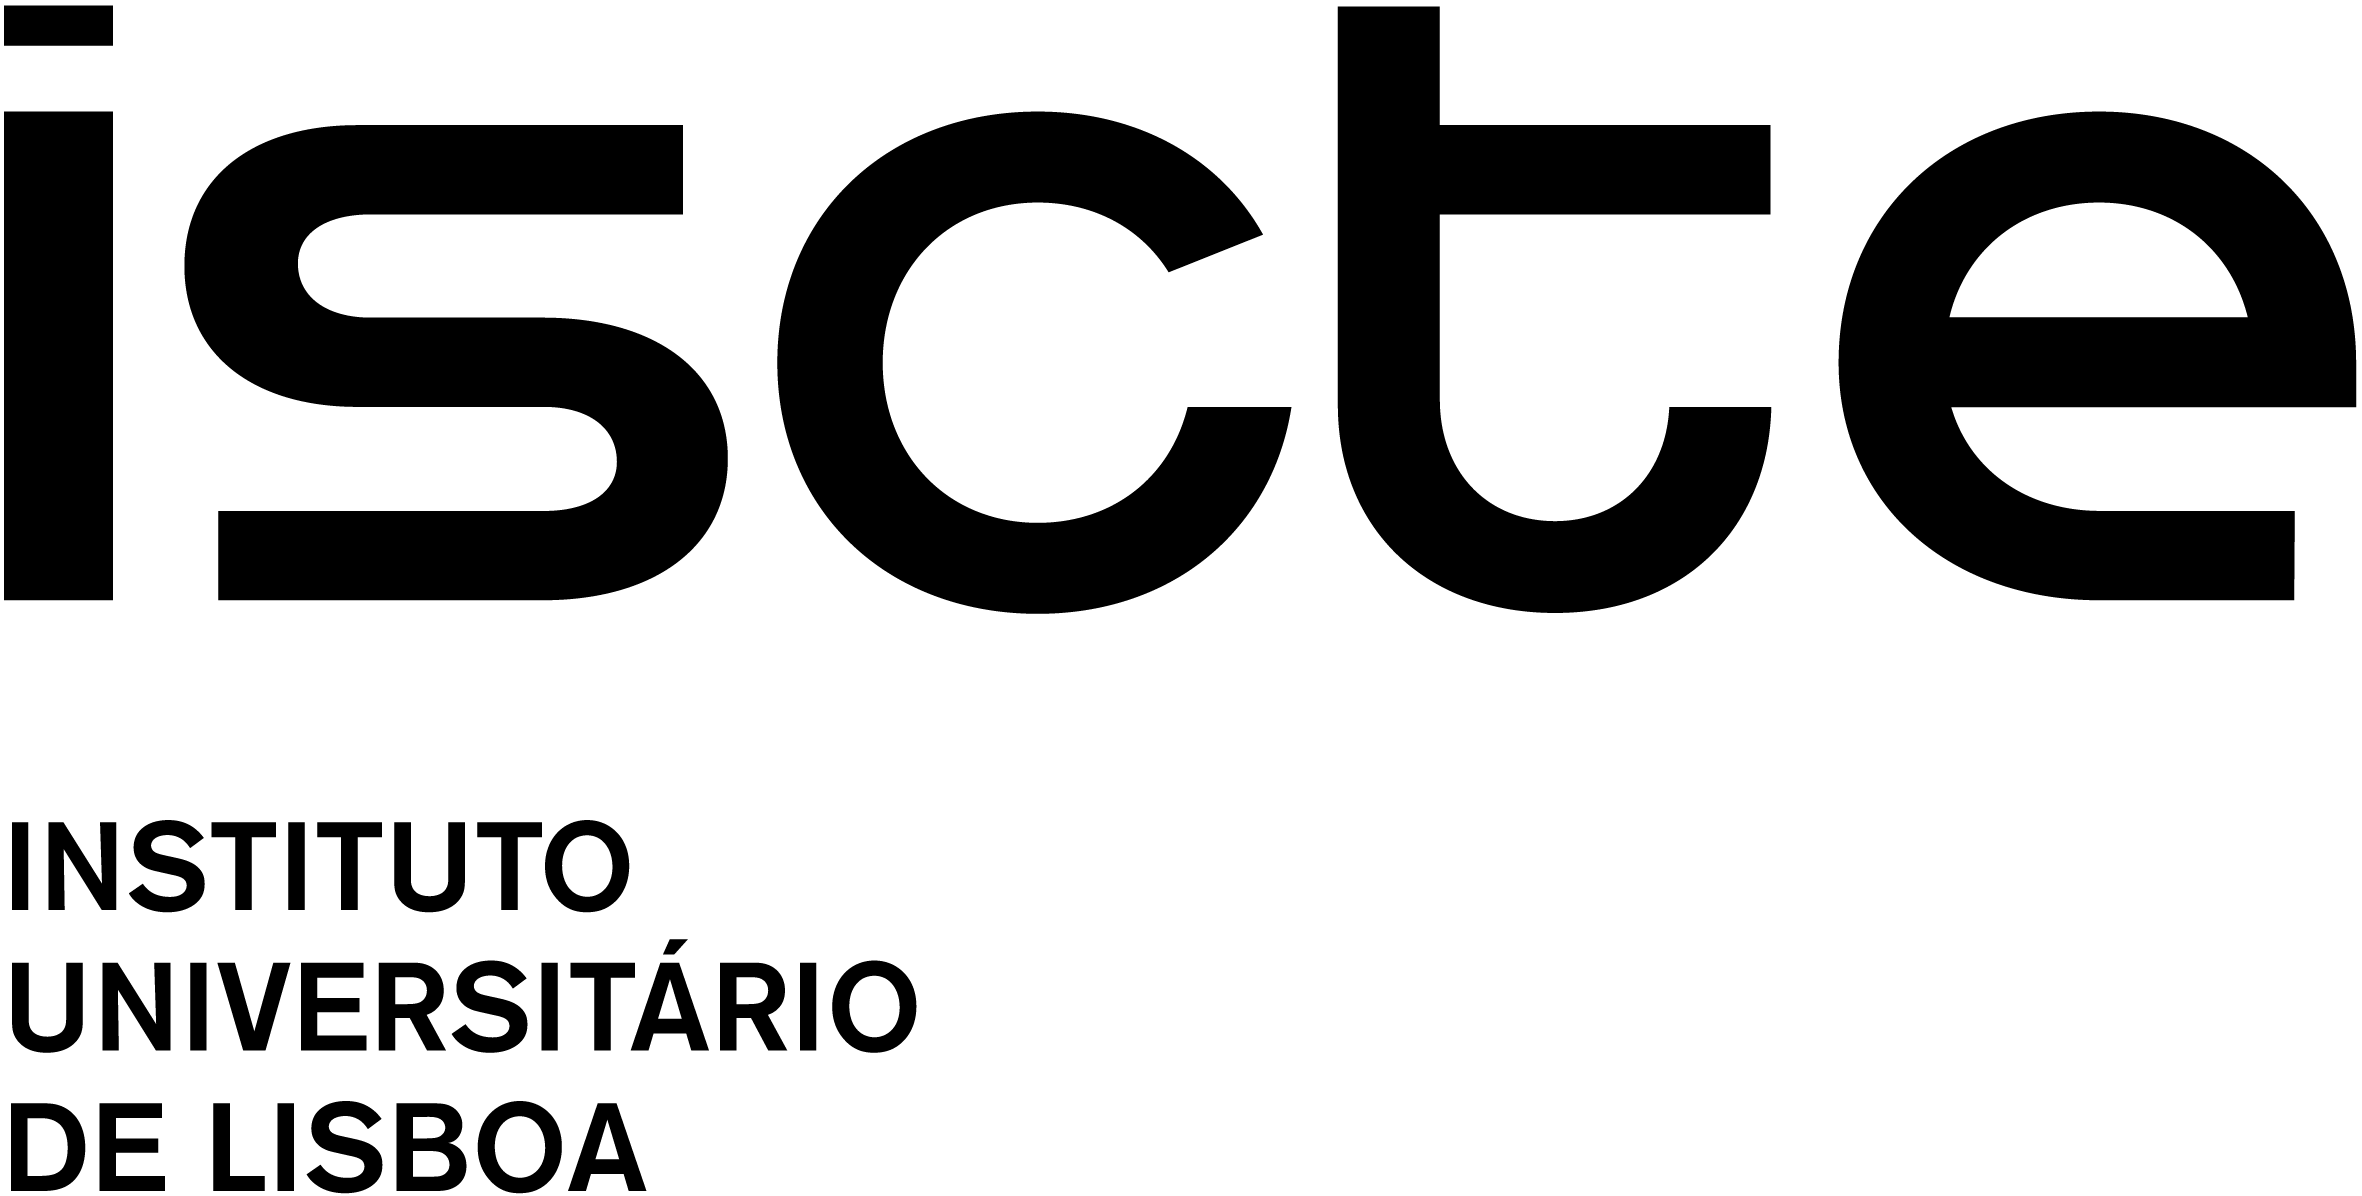
\includegraphics[width=6.03cm]{imagens/iscte}\\[3.3mm]

\hrulefill
~\\
~\\
~\\
\textbf{Título}\\
~\\
~\\
~\\
~\\
\textit{name}\\
~\\
~\\
~\\
Master in Computer Engineering\\
~\\
~\\
~\\
Supervisor:\\
Doctor \textit{name}, \textit{category} Professor,\\
Iscte -- Instituto Universitário de Lisboa\\
~\\
~\\
~\\
Co-Supervisor:\\
Doctor \textit{name}, \textit{category} Professor,\\
\textit{instituição}\\
~\\
~\\
~\\
~\\
October, 2022
\end{flushleft}
\thispagestyle{empty}
\cleardoublepage
\begin{flushleft}
  
\includegraphics[width=6.03cm]{imagens/ista}\\[7mm]
\hrulefill
~\\
~\\
~\\
Department of Information Science and Technology\\
~\\
~\\
\textbf{Título}\\
~\\
~\\
~\\
~\\
\textit{name}\\
~\\
~\\
~\\
Master in Computer Engineering\\
~\\
~\\
~\\
Supervisor:\\
Doctor \textit{name}, \textit{category} Professor,\\
Iscte -- Instituto Universitário de Lisboa\\
~\\
~\\
~\\
Co-Supervisor:\\
Doctor \textit{name}, \textit{category} Professor,\\
\textit{university}\\
~\\
~\\
~\\
~\\
October, 2022
  \end{flushleft}
  \thispagestyle{empty}
\rmfamily
\normalsize
\frontmatter
%\addtocontents{toc}{\setcounter{tocdepth}{2}}
\thispagestyle{empty}

\frontmatter
\addtocontents{toc}{\setcounter{tocdepth}{2}}
\thispagestyle{empty}

\begin{dedication}%

\begin{flushright}
\textit{Write here your dedication}
\end{flushright}%
\end{dedication}

\setcounter{page}{1}
\pagenumbering{roman} %
\chapter*{Acknowledgment}

Write here the acknowledgments and grants, if any

\chapter*{Resumo}

Escrever aqui o resumo em Português.

\vspace{3ex}
\textsc{Palavras Chave:} \textit{palavra\_1}, \textit{palavra\_2}, \dots

\chapter*{Abstract}

Write here your abstract in English.

\vspace{3ex}
\textsc{Keywords:} \textit{word\_1}, \textit{word\_2}, \dots

\tableofcontents
\listoffigures
\listoftables
\cleardoublepage
%\printglossary[type=\acronymtype, nonumberlist, nogroupskip]
\chapter*{List of Acronyms}
\begin{acronym}
 \acro{AI}{Artificial Intelligence}
 \acro{ML}{Machine Learning}
\end{acronym}

\mainmatter

\hyphenation{wri-te he-re pro-per hy-phe-ni-za-tion
}%

\setcounter{page}{1} \pagenumbering{arabic}

\chapter{Introduction}
\label{ch:introduction}

% O primeiro parágrafo de cada secção ou capítulo não deve ser indentado.
\noindent Newell et al.~\cite{newell:et:al:1958} present a seminal work in \ac{AI}.

Table~\ref{tab:my_label_1} shows a beautiful table. This beautiful table has two columns, both centered, and two rows. The numbering restarts in each chapter, but includes the chapter number.

\begin{table}[htb]
    \caption{Tables' captions should always appear on the top of the table}
    \label{tab:my_label_1}
    \begin{tabular}{c|c}
         H1 & H2 \\\hline
         v1 & v2
    \end{tabular}
\end{table}

Nowadays, what it is recognized as \ac{AI} is mostly \ac{ML}.

\section{Document Structure}
\label{sect:docstruct}

\noindent This document is structured as follows.

\chapter{Conclusion}
\label{ch:conclusion}

\noindent Figure~\ref{fig:my_label} shows the logo of the Iscte school responsible for this master program.

\begin{figure}[hbt]
    
\includegraphics[width=.42\columnwidth]{imagens/ista.png}
    \caption{Figures' captions should always appear on the bottom of the figure}
    \label{fig:my_label}
\end{figure}

Table~\ref{tab:my_label_2} shows the same beautiful table of Chapter~\ref{ch:introduction}, but, as we can see, it has now the number \ref{tab:my_label_2}, as expected.

\begin{table}[htb]
    \caption{Tables' captions should always appear on the top of the table}
    \label{tab:my_label_2}
    \begin{tabular}{c|c}
         H1 & H2 \\\hline
         v1 & v2
    \end{tabular}
\end{table}

\printbibliography[title={References}]
%\printbibliography[title={Bibliografia}] % PT

\end{document}
